\uuid{Kush}
\titre{Egalité à une série de Fourier}
\theme{séries de Fourier}
\auteur{}
\datecreate{2024-06-13}
\organisation{AMSCC}
\contenu{

\texte{ Soit $f:\R\rightarrow \R$, impaire, $2\pi$-p\'eriodique, d\'efinie par $f(x)=1$ pour tout $x\in]0,\pi[ $. }
\begin{enumerate}
	\item \question{ Dessiner le graphe de $f$. Quelle est la r\'egularit\'e de $f$ ? }
	\reponse{
		\begin{center}
			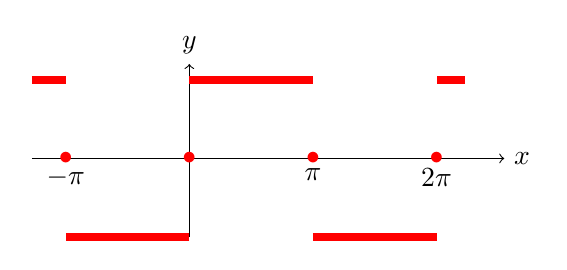
\begin{tikzpicture}[xscale=0.5]
				\draw[->] (-4,0) -- (8,0);
				\draw (8,0) node[right] {$x$};
				\draw (6.28,0) node[below] {$2\pi$};
				\draw (3.14,0) node[below] {$\pi$};
				\draw (-3.14,0) node[below] {$-\pi$};
				\draw [->] (0,-1) -- (0,1.2);
				\draw (0,1.2) node[above] {$y$};
				\draw[line width=3pt, color=red] (7,1) -- (6.28,1);
				\draw[line width=3pt, color=red] (3.14,-1) -- (6.28,-1);
				\draw[line width=3pt, color=red] (0,1) -- (3.14,1);
				\draw[color=red] (0,0) node {$\bullet$} ;
				\draw[color=red] (-3.14,0) node {$\bullet$} ;
				\draw[color=red] (3.14,0) node {$\bullet$} ;
				\draw[color=red] (6.28,0) node {$\bullet$} ;
				\draw[line width=3pt, color=red] (0,-1) -- (-3.14,-1);
				\draw[line width=3pt, color=red] (-4,1) -- (-3.14,1);
			\end{tikzpicture}
		\end{center}
		La fonction $f$ est continue par morceaux, discontinue aux points $(k\pi), \, k\in \Z$. Elle est impaire donc $f(0)=0$.
	}
	\item \question{ D\'eterminer les coefficients de Fourier trigonom\'etriques de $f$. }
	\reponse{La fonction $f$ étant impaire, les coefficients de Fourier $a_n(f)$ sont nuls et : 
		\begin{align*}
			b_n(f) &= \frac{2}{\pi} \int_0^{\pi} f(t)\sin(nt)\mathrm{d}t \\
			&= \frac{2}{\pi} \int_0^{ {\pi}} \sin(nt)\mathrm{d}t \\
			&= \frac{2}{\pi} \left[-\frac{1}{n}\cos(nt)\right]_0^{ {\pi}} \\
			&= \frac{2}{n\pi}\left(1-\cos\left({n\pi}\right)\right)\\
			&= \frac{2}{n\pi}\left(1-(-1)^n\right)
		\end{align*}	
		La série de Fourier est donc $\displaystyle S_n(f) = \sum_{n\geq 1} \frac{2}{n\pi}\left(1-(-1)^n\right)\sin(nx) = \sum_{k \geq 0} \frac{4}{(2k+1)\pi}\sin((2k+1)x)$. }
	\item \question{ Calculer les sommes :
	$$\sum_{n=0}^{+\infty} \frac{(-1)^n }{2n+1 } \qquad \text{ et } \qquad  \sum_{n=0}^{+\infty} \frac{1 }{(2n+1)^2 }.$$ }
	\reponse{La fonction $f$ étant continue en $\frac{\pi}{2}$, d'après le théorème de Dirichlet on a :
		$$f\left(\frac{\pi}{2}\right) = \sum_{k=0}^{+\infty }	\frac{4}{(2k+1)\pi}\sin\left((2k+1)\frac{\pi}{2}\right) = \sum_{k=0}^{+\infty }	\frac{4}{(2k+1)\pi} \times (-1)^k$$
		d'où $\sum_{n=0}^{+\infty} \frac{(-1)^n }{2n+1 } = \frac{4}{\pi}$. 
		
		D'après la formule de Parseval,
		$$\frac{1}{2\pi}\int_0^{2\pi}f(t)^2 \mathrm{d}t = 0 + \frac{1}{2} \sum_{k=0}^{+\infty }	\left(\frac{4}{(2k+1)\pi}\right)^2$$
		Or par définition de $f$, $\frac{1}{2\pi}\int_0^{2\pi}f(t)^2 \mathrm{d}t = \frac{1}{2\pi}\int_0^{2\pi}1 \mathrm{d}t = 1$ donc $\displaystyle \sum_{n=0}^{+\infty} \frac{1 }{(2n+1)^2 } = 2 \times \frac{\pi^2}{4^2} = \frac{\pi^2}{8}$. 
	}
	\item \question{ En d\'eduire la valeur exacte de  $ \displaystyle  \sum_{n=1}^{+\infty} \frac{1 }{n^2 }$. }
	\reponse{On remarque que 
		\begin{align*} \sum_{n=1}^{+\infty} \frac{1 }{n^2 } &= \sum_{k=1}^{+\infty} \frac{1 }{(2k)^2} + \sum_{k=0}^{+\infty} \frac{1 }{(2k+1)^2} \\
			&= \frac{1}{4} \sum_{k=1}^{+\infty} \frac{1 }{k^2} + \frac{\pi^2}{8}
		\end{align*}
		d'où $\frac{3}{4} \sum_{n=1}^{+\infty} \frac{1 }{n^2 } = \frac{\pi^2}{8}$ d'où $$\sum_{n=1}^{+\infty} \frac{1 }{n^2 } = \frac{\pi^2}{6}$$
	}
	%\qquad \text{ et } \qquad  
	%\sum_{n=1}^{+\infty} \frac{(-1 )^n }{n^2 }.
	%\]
\end{enumerate}
}